\section{Experimental Setup and Measurements}
\label{sec:procedure}
In this experiment, a Sagnac interferometer is utilized for the measurements. 
This type of interferometer is especially stable compared to other types
of interferometers, such as the Mach-Zehnder or Michelson interferometer, due to
both beams following the same path.

\begin{figure}
    \centering
    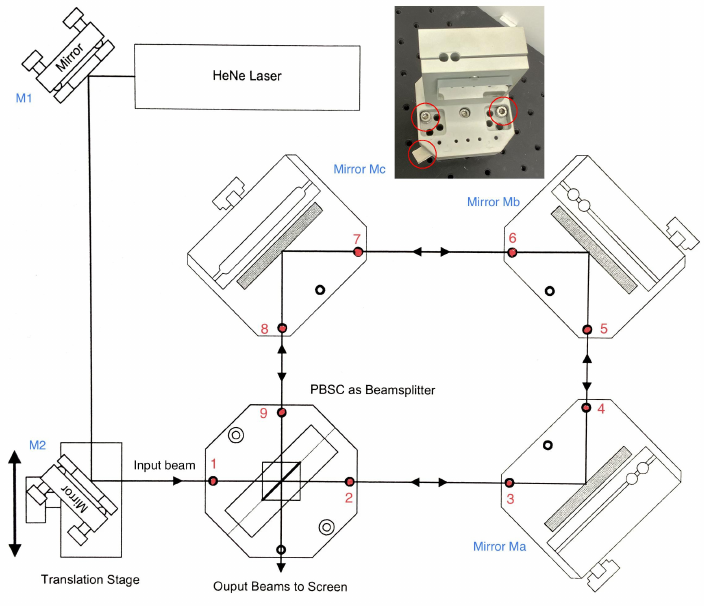
\includegraphics[width=0.7\textwidth]{pictures/Sagnac.png}
    \caption{Schematic representation of the Sagnac interferometer setup. \cite{V64}}
    \label{fig:sagnac}
\end{figure}

The Sagnac interferometer used in this experiment is schematically depicted in Figure \ref{fig:sagnac}. 
A Helium-Neon Laser, emitting light at a wavelength of $\lambda_\text{Laser} = \SI{632.99}{\nano\meter}$, 
serves as the coherent light source. The laser beam, after being reflected by adjustment mirrors M1 and M2, 
traverses a polarization filter before being split by the PBSC, as detailed 
in Section \ref{sec:interference}. The polarization filter regulates the intensities of the s- and p-polarized 
beams emitted from the PBSC. An equal intensity for both beams is achieved at a $\SI{45}{\degree}$ angle 
of the polarization filter. The beams, one following a clockwise path and the other counterclockwise, are 
then reflected by mirroThey re-converge at the PBSC to form the output beam, 
which is split by another PBSC to be able to measure 
the s- and p-polarized parts of the beam sperately.rs Ma, Mb, and Mc. 
They re-converge at the PBSC to form the output beam. 
This beam is then split by another PBSC, 
which allows for separate measurement of the s- and p-polarized components of the beam.


\subsection{Alignment of the Sagnac Interferometer}
The initial step in aligning the Sagnac Interferometer involves centering the laser beam on mirrors M1 and M2. 
These mirrors are crucial for directing the beam precisely through the center of the PBSC. 
Utilizing adjustment plates, the beam path is fine-tuned so that the laser strikes mirrors Ma and Mc centrally. 
Subsequent adjustments ensure both beams converge at the center of mirror Mb. 
Proper alignment is indicated when both beams rejoin in the PBSC. 
The quality of this alignment is gauged by observing the interference pattern of the output beam, with the 
polarization filter set to $\SI{45}{\degree}$. 
The presence of fringes in this pattern signals phase differences due to path variations, necessitating 
further adjustments to ensure the beams are perfectly parallel throughout the entire interferometer.

\subsection{Measurement of the Contrast}
\label{sec:contrast}
To assess the contrast of the interference pattern, a rotating glass plane holder is positioned within the 
beam's path. 
The contrast is measured as a function of the polarization angle, varying the direction of the polarization 
filter in \SI{5}{\degree} increments across a range of \SIrange{0}{180}{\degree}. 
A diode, by recording the voltage, measures the intensities of the minima and maxima in the interference pattern. 
Fine-tuning of these minima and maxima is achieved through adjustments made to the rotating glass plane holder.

For subsequent measurements, the polarization filter is set to an angle that maximizes the contrast, ensuring 
optimal conditions for accurate data collection.

\subsection{Measurement of the Refractive Index of Glass}
\label{sec:measurement_glass}
The refractive index of glass is measured using two diodes connected to a Modern Interferometry Controller. 
This device is designed to count the occurrences of intensity minima and maxima. 
The procedure involves gradually rotating the glass holder from \SIrange{0}{8}{\degree}, and at each 
\SI{2}{\degree} increment, the count of maxima is recorded. 

\subsection{Measurement of the Refractive Index of Gas}
\label{sec:measurement_gas}
The refractive index of air in the laboratory is determined as a function of pressure. 
A gas cell, with a length of $L = \SI{100 \pm 0.1}{\milli\meter}$, is inserted into the beam path to 
facilitate this measurement. 
Starting from a vacuum, the pressure inside the cell is incrementally increased. 
The count of intensity minima and maxima is recorded in steps of \SI{50}{\milli\bar}.
